\documentclass[journal,12pt,twocolumn]{IEEEtran}
%
\usepackage{setspace}
\usepackage{gensymb}
\usepackage{xcolor}
\usepackage{polynom}
\usepackage{caption}
%\usepackage{subcaption}
%\doublespacing
\singlespacing

%\usepackage{graphicx}
%\usepackage{amssymb}
%\usepackage{relsize}
\usepackage[cmex10]{amsmath}
\usepackage{mathtools}
%\usepackage{amsthm}
%\interdisplaylinepenalty=2500
%\savesymbol{iint}
%\usepackage{txfonts}
%\restoresymbol{TXF}{iint}
%\usepackage{wasysym}
\usepackage{hyperref}
\usepackage{amsthm}
\usepackage{mathrsfs}
\usepackage{txfonts}
\usepackage{stfloats}
\usepackage{cite}
\usepackage{cases}
\usepackage{subfig}
%\usepackage{xtab}
\usepackage{longtable}
\usepackage{multirow}
%\usepackage{algorithm}
%\usepackage{algpseudocode}
%\usepackage{enumerate}
\usepackage{enumitem}
\usepackage{mathtools}
%\usepackage{iithtlc}
%\usepackage[framemethod=tikz]{mdframed}
\usepackage{listings}

\let\vec\mathbf
\newcommand{\myvec}[1]{\ensuremath{\begin{pmatrix}#1\end{pmatrix}}}

%\usepackage{stmaryrd}


%\usepackage{wasysym}
%\newcounter{MYtempeqncnt}
\DeclareMathOperator*{\Res}{Res}
%\renewcommand{\baselinestretch}{2}
\renewcommand\thesection{\arabic{section}}
\renewcommand\thesubsection{\thesection.\arabic{subsection}}
\renewcommand\thesubsubsection{\thesubsection.\arabic{subsubsection}}

\renewcommand\thesectiondis{\arabic{section}}
\renewcommand\thesubsectiondis{\thesectiondis.\arabic{subsection}}
\renewcommand\thesubsubsectiondis{\thesubsectiondis.\arabic{subsubsection}}

%\renewcommand{\labelenumi}{\textbf{\theenumi}}
%\renewcommand{\theenumi}{P.\arabic{enumi}}

% correct bad hyphenation here
\hyphenation{op-tical net-works semi-conduc-tor}

\lstset{
language=Python,
frame=single, 
breaklines=true,
columns=fullflexible
}



\begin{document}
%

\theoremstyle{definition}
\newtheorem{theorem}{Theorem}[section]
\newtheorem{problem}{Problem}
\newtheorem{proposition}{Proposition}[section]
\newtheorem{lemma}{Lemma}[section]
\newtheorem{corollary}[theorem]{Corollary}
\newtheorem{example}{Example}[section]
\newtheorem{definition}{Definition}[section]
%\newtheorem{algorithm}{Algorithm}[section]
%\newtheorem{cor}{Corollary}
\newcommand{\BEQA}{\begin{eqnarray}}
\newcommand{\EEQA}{\end{eqnarray}}
\newcommand{\define}{\stackrel{\triangle}{=}}
\bibliographystyle{IEEEtran}
%\bibliographystyle{ieeetr}
\providecommand{\nCr}[2]{\,^{#1}C_{#2}} % nCr
\providecommand{\nPr}[2]{\,^{#1}P_{#2}} % nPr
\providecommand{\mbf}{\mathbf}
\providecommand{\pr}[1]{\ensuremath{\Pr\left(#1\right)}}
\providecommand{\qfunc}[1]{\ensuremath{Q\left(#1\right)}}
\providecommand{\sbrak}[1]{\ensuremath{{}\left[#1\right]}}
\providecommand{\lsbrak}[1]{\ensuremath{{}\left[#1\right.}}
\providecommand{\rsbrak}[1]{\ensuremath{{}\left.#1\right]}}
\providecommand{\brak}[1]{\ensuremath{\left(#1\right)}}
\providecommand{\lbrak}[1]{\ensuremath{\left(#1\right.}}
\providecommand{\rbrak}[1]{\ensuremath{\left.#1\right)}}
\providecommand{\cbrak}[1]{\ensuremath{\left\{#1\right\}}}
\providecommand{\lcbrak}[1]{\ensuremath{\left\{#1\right.}}
\providecommand{\rcbrak}[1]{\ensuremath{\left.#1\right\}}}
\theoremstyle{remark}
\newtheorem{rem}{Remark}
\newcommand{\sgn}{\mathop{\mathrm{sgn}}}
\providecommand{\abs}[1]{\left\vert#1\right\vert}
\providecommand{\res}[1]{\Res\displaylimits_{#1}} 
\providecommand{\norm}[1]{\lVert#1\rVert}
\providecommand{\mtx}[1]{\mathbf{#1}}
\providecommand{\mean}[1]{E\left[ #1 \right]}
\providecommand{\fourier}{\overset{\mathcal{F}}{ \rightleftharpoons}}
\providecommand{\ztrans}{\overset{\mathcal{Z}}{ \rightleftharpoons}}
%\providecommand{\hilbert}{\overset{\mathcal{H}}{ \rightleftharpoons}}
\providecommand{\system}{\overset{\mathcal{H}}{ \longleftrightarrow}}
	%\newcommand{\solution}[2]{\textbf{Solution:}{#1}}
\newcommand{\solution}{\noindent \textbf{Solution: }}
\providecommand{\dec}[2]{\ensuremath{\overset{#1}{\underset{#2}{\gtrless}}}}
\numberwithin{equation}{section}
%\numberwithin{equation}{subsection}
%\numberwithin{problem}{subsection}
%\numberwithin{definition}{subsection}
\makeatletter
\@addtoreset{figure}{problem}
\makeatother
\let\StandardTheFigure\thefigure
%\renewcommand{\thefigure}{\theproblem.\arabic{figure}}
\renewcommand{\thefigure}{\theproblem}
%\numberwithin{figure}{subsection}
\def\putbox#1#2#3{\makebox[0in][l]{\makebox[#1][l]{}\raisebox{\baselineskip}[0in][0in]{\raisebox{#2}[0in][0in]{#3}}}}
     \def\rightbox#1{\makebox[0in][r]{#1}}
     \def\centbox#1{\makebox[0in]{#1}}
     \def\topbox#1{\raisebox{-\baselineskip}[0in][0in]{#1}}
     \def\midbox#1{\raisebox{-0.5\baselineskip}[0in][0in]{#1}}
\vspace{3cm}

\title{\LARGE{PINGALA ASSIGNMENTS}}
\author{\normalsize J Sai Sri Hari Vamshi\\ \footnotesize AI21BTECH11014}
\date{}
\maketitle
\tableofcontents
\renewcommand{\thefigure}{\theenumi}
\renewcommand{\thetable}{\theenumi}
\bigskip    

\section{JEE 2019}
\noindent Let $\alpha$ and $\beta$ ($\alpha > \beta$) be the roots of the equation $z^2-z-1=0$. Define,

\begin{align}
	a_n & = \frac{\alpha^n-\beta^n}{\alpha-\beta}, \quad n \ge 1\\
	b_n & = a_{n-1} - a_{n+1}, \quad n \ge 2, \quad b_1 = 1
\end{align}

\noindent Verify the following using a python code.

\begin{enumerate}[label=\thesection.\arabic*,ref=\thesection.\theenumi]
	
	Download the Python code using
	
	\begin{lstlisting}
		wget https://https://github.com/HARI-donk-EY/sig_pros/tree/main/pingala/codes/1.py
	\end{lstlisting}

	and run it using,
	
	\begin{lstlisting}
		$python3 1.py
	\end{lstlisting}
	
	\item
	\begin{align}
     		\sum_{k=1}^na_k = a_{n+2}-1, \quad n \ge 1
	\end{align}
	
	\solution\\
	From Fig. \ref{fig:1.1}, both the graphs are similar for $LHS$ and $RHS$.\\ 
	Hence 1.1 is true.

	\begin{figure}[ht]
		\begin{center}
			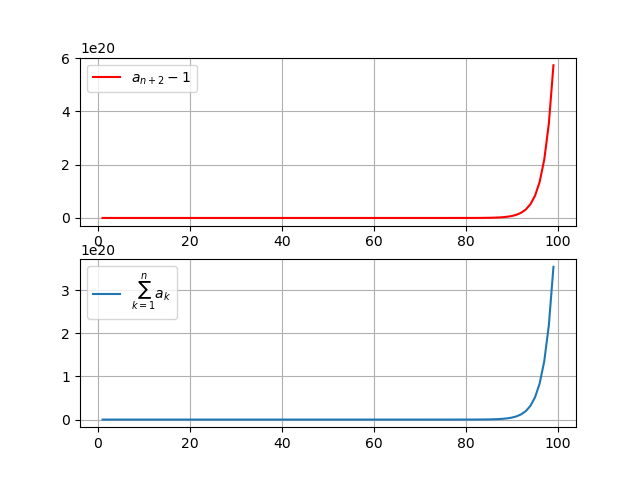
\includegraphics[width=0.7\columnwidth]{figs/1_1}
		\end{center}
		\captionof{figure}{}
		\label{fig:1.1}    
	\end{figure}
		
	\item 
	\begin{align}
     		\sum_{k=1}^\infty\frac{a_k}{10^k} = \frac{10}{89}
	\end{align}

	\solution
	The Fig. \ref{fig:1.2} shoes that the difference between $LHS$ and $RHS$ tens to zero as the value of $k$ increases.\\
	It shows that for a large value of $k$, the
	\begin{align*}
		LHS \to RHS	
	\end{align*}
	Hence 1.2 is true.

	\begin{figure}[ht]
		\begin{center}
			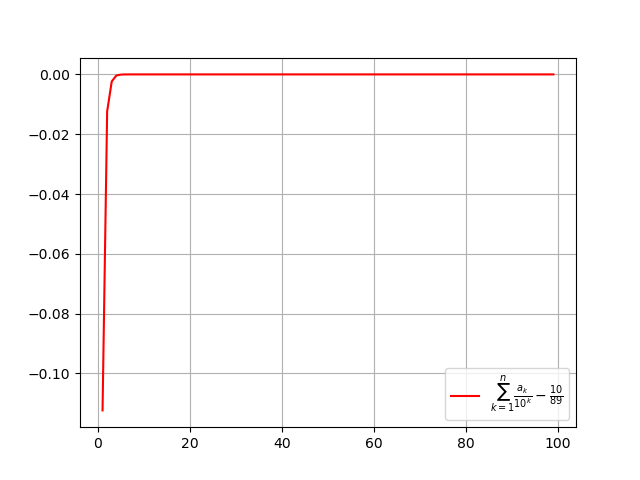
\includegraphics[width=0.7\columnwidth]{figs/1_2}
		\end{center}
		\captionof{figure}{}
		\label{fig:1.2}    
	\end{figure}

	\item 
	\begin{align}
    	 	b_n = \alpha^n + \beta^n, \quad n \ge 1
	\end{align}

	\solution	
	From Fig. \ref{fig:1.3}, both the graphs are similar for $LHS$ and $RHS$.\\ 
	Hence 1.3 is true.

	\begin{figure}[ht]
		\begin{center}
			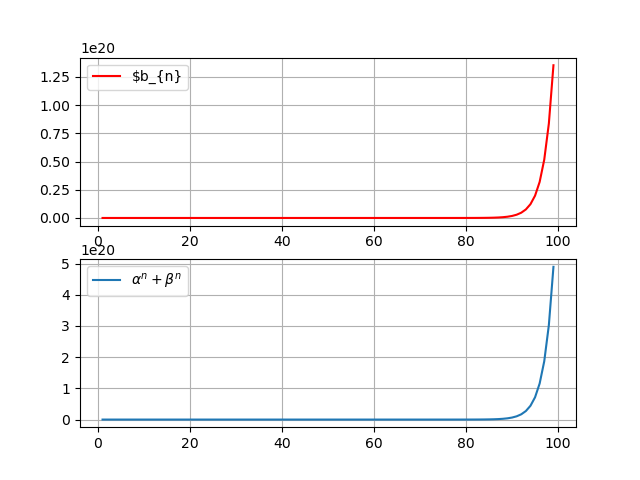
\includegraphics[width=0.7\columnwidth]{figs/1_3}
		\end{center}
		\captionof{figure}{}
		\label{fig:1.3}    
	\end{figure}

	\item 
	\begin{align}
     		\sum_{k=1}^\infty\frac{b_k}{10^k}=\frac{8}{89}
	\end{align}

	\solution\\ 
	The Fig. \ref{fig:1.4} shoes that the difference between $LHS$ and $RHS$ tends to $\frac{12}{89}$ as the value of $k$ increases.\\
	It shows that for a large value of $k$, the
	\begin{align*}
		LHS \nrightarrow RHS	
	\end{align*}
	Hence 1.4 is false.

	\begin{figure}[ht]
		\begin{center}
			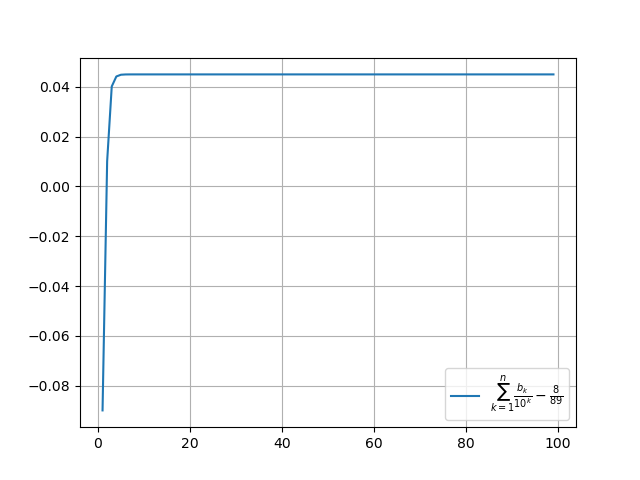
\includegraphics[width=0.7\columnwidth]{figs/1_4}
		\end{center}
		\captionof{figure}{}
		\label{fig:1.4}    
	\end{figure}
\end{enumerate}

\section{}
\begin{enumerate}[label=\thesection.\arabic*,ref=\thesection.\theenumi]
	
	\item 

\end{enumerate}

\end{document}
